
\documentclass[12pt,journal,compsoc]{IEEEtran}
\usepackage[spanish]{babel}
\usepackage{array}
\usepackage{graphicx}
\usepackage{diagbox}
\usepackage{float}
\usepackage[utf8]{inputenc}
\newcommand\MYhyperrefoptions{bookmarks=true,bookmarksnumbered=true,
pdfpagemode={UseOutlines},plainpages=false,pdfpagelabels=true,
colorlinks=true,linkcolor={black},citecolor={black},urlcolor={black},
pdftitle={Relación entre la legibilidad de una serie de libros y sus respectivas calificaciones},
pdfsubject={Neurociencia},
pdfauthor={Sabrina Izcovich, Roberto Rama, Gustavo Juantorena},
pdfkeywords={Neurociencia, Vocabulario, Libro, Métricas, Legibilidad}}

\begin{document}
\title{Relación entre la legibilidad de libros y sus respectivas calificaciones}

\author{Gustavo~Juantorena~~~~~~
        Roberto~Rama~~~~~~
        Sabrina~Izcovich\\
        \textit{Facultad de Ciencias Exactas, UBA}}


\IEEEtitleabstractindextext{

\begin{abstract}
En la actualidad, el avance de la tecnología permite compartir experiencias de distinta índole entre sus usuarios. Por ejemplo, el intercambio de críticas y comentarios sobre diferentes productos, que pueden ocasionar un aumento o disminución de sus respectivas ventas. Es por esto que conocer los motivos de los usuarios a la hora de calificar resulta útil cuando se desea estudiar el mercado. En este trabajo, analizamos libros en base al nivel de legibilidad de los mismos demostrando relaciones entre éste y la valoración que reciben. Para ello, aplicamos diversas métricas clásicas de legibilidad a un subconjunto de libros extraídos de la base de datos de Amazon.
\end{abstract}

% cita en ``puntaje numerico comparativo a una obra''

\begin{IEEEkeywords}
Neurociencia, Métricas, Legibilidad, Libros, Reseñas.
\end{IEEEkeywords}}

\maketitle
\IEEEdisplaynontitleabstractindextext
\IEEEpeerreviewmaketitle

\section{Introducción}
\IEEEPARstart{D}{esde} siempre, las personas han expresado diferentes gustos y opiniones sobre diversos tópicos, siendo la literatura uno de los más discutidos. Los fundamentos de las opiniones pueden ser muy variados e incluso difusos para los dueños de las mismas. Otras veces, los mismos pueden estar influenciados por la opinión del resto de los usuarios\cite{muchnik} o ser poco objetivos debido a experiencias personales (la mayoría de los usuarios sólo da una reseña cuando su relación con el producto es muy buena o muy mala\cite{hu}). A pesar de esto, las calificaciones que los usuarios asignan en los sitios web tienden a converger a un valor mayormente positivo con el transcurso del tiempo\cite{zhang}; y aunque en general el comportamiento de éstas sigue siendo una incógnita, existen estudios que afirman se trata de una distribución binomial\cite{hu}. Sin embargo, no todo comportamiento puede ser justificado por una tendencia\cite{zhang}, por lo que su estudio sigue siendo valioso. 

En nuestro análisis, buscamos responder a la pregunta de si la legibilidad de los libros impacta de alguna forma en las reseñas que los usuarios asignan. Para esto, suponemos que los libros más faciles de leer, o sea más legibles, tienden a tener mejor puntaje que aquellos que resultan más difíciles. Para demostrar nuestra hipótesis, recompilamos una amplia variedad de libros de distintos autores, géneros y formatos, junto con la información de las calificaciones asignadas por sus lectores. Ésta última fue extraída de la base de datos de Amazon\footnote{http://snap.stanford.edu/data/amazon-meta.html}, utilizada también en un análisis de marketing viral\cite{leskovec}. Intentamos que los libros analizados conformaran un conjunto de datos homogéneo para evitar sesgos ocasionados por una categoría o autor en particular.

A pesar del gran esfuerzo en el área lingüística para introducir criterios computacionales que modelen y evalúen legibilidad, un esquema representativo y concluyente todavía se encuentra en falta \cite{orlow, klare, kanungo, karmakar}. Por esto, y ya que los resultados entre distintas métricas clásicas pueden no ser consistentes\cite{izgi}, utilizamos un conjunto de las mismas para medir la legibilidad y contrastar los resultados. De esta manera, al observar la misma tendencia para distintas métricas, podremos evidenciar la validez de los resultados. Hubiese sido óptimo utilizar métricas más avanzadas para la experimentación como \textit{Coh-Metrix}\cite{graesser}, que parece tener una consistencia y utilidad mayores a las métricas básicas\cite{crossley}, pero no estaban disponibles para hacer de su uso fácilmente.

Finalmente, el trabajo de \textit{Diuk, C. G., et. al., 2012} \cite{diuk}, resultó de gran inspiración sobre la potencialidad del análisis de grandes repositorios de datos con el fin de hacer predicciones. En el mismo, se utilizaron textos de distintas épocas en orden cronológico con el fin de probar si el constructo introspección creció o disminuyó a lo largo de los años.

En la seccion ... %TODO: Completar al final
En primer lugar, se explicará el proceso realizado a lo largo del estudio y las herramientas empleadas detalladamente, incluyendo el criterio de clasificación de los libros y sus puntajes, como también las métricas empleadas. Luego, se expondrán los resultados empíricos obtenidos por categoría y la correlación entre éstos. Más tarde, presentaremos un análisis estadístico de los resultados medidos que nos permitirán, finalmente, extraer conclusiones.

% los usuarios solo escriben reviews cuando su relacion con el producto es muy buena o muy mala \cite{hu}
% identifica el raiting como la diferencia entre la calidad real del producto y lo que esperaba el usuario \cite{talwar}
% votos positivos crean un efecto positivo mientras que los votos negativos crean un efecto de correccion\cite{muchnik}
% el puntaje de reseña en los sitios normalmente es muy alto \cite{chevalier, fowler}
% los puntajes de reseña tienden a converger a números altos\cite{zhang}

\section{Métricas}

Las métricas de legibilidad son fórmulas que sirven para evaluar la legibilidad de un texto de forma automática, normalmente utilizadas como reemplazo de una encuesta con humanos. Las métricas analizadas en el presente trabajo fueron diseñadas entre los años 1940 a 1970, por lo que muchas veces debían ser calculadas por máquinas simples o humanos. A pesar de haber pasado mucho tiempo desde su creación, las métricas clásicas siguen siendo utilizadas en muchos estudios y hasta aparecen como condiciones necesarias legales en, por ejemplo, la creación de las pólizas de seguros automotrices. Las métricas estudiadas, exceptuando Flesch–Kincaid Reading Ease, simbolizan en sus valores la edad promedio o nivel educativo necesarios para entender el texto analizado con ésta. %lo de automotrices es en USA o aca tambien?

\subsection{ARI}

El índice de legibilidad automatizado (\textbf{ARI})\cite{ari-flesch} fue diseñado a pedido de las fuerzas aéreas de los Estados Unidos con el propósito de monitorear en tiempo real la legibilidad de los textos producidos por máquinas de escribir eléctricas. A diferencia de otros índices, junto con el Coleman-Liau, ARI se basa en un factor de caracteres por palabra en vez de sílabas por palabra. Aunque la opinión sobre la pérdida de precisión en el índice con uso de este factor varía, suele ser más rápido de calcular ya que es más fácil contar cantidad de caracteres que de sílabas\cite{liang}.

El índice de legibilidad automatizado posee dos variables: caracteres por palabra y palabras por frase. El resultado corresponde al grado académico en los Estados Unidos. Su fórmula se define como:

$$ARI = 4.71\cdot \frac{caracteres}{palabras}+0.5\cdot \frac{palabras}{frases} - 21.43$$

donde \textit{caracteres} corresponde a la cantidad de letras y números, \textit{palabras} es la cantidad de espacios y \textit{frases} la cantidad de frases.

\subsection{Coleman-Liau index}

El índice \textbf{Coleman-Liau}\cite{coleman-liau} fue diseñado para ser calculable de forma mecánica a partir de textos impresos. Dado que sólo requiere analizar los caracteres por palabra, podría ser usado en conjunto con escáneres mecánicos simples que sólo necesiten reconocer caracteres, palabras y límites de oraciones, eliminando la necesidad de un reconocimiento completo de caracteres. %no entiendo esta frase!
La fórmula del mismo se define como:

$$CLI = 5.88 \cdot \frac{letras}{palabras} - 29.6 \cdot \frac{frases}{palabras} - 15.8$$

\subsection{Flesch–Kincaid}
Las fórmulas de legibilidad \textbf{Flesch–Kincaid Reading Ease}\cite{ari-flesch} y \textbf{Flesch–Kincaid Grade Test} fueron diseñadas bajo el pedido de la marina de los Estados Unidos para evaluar la dificulad de los manuales técnicos, antes de que el Grade Test se vuelva un estándar en la milicia. Ambas fórmulas se correlacionan casi de forma inversa, lo que resulta coherente dado que usan las mismas medidas (relación entre sílabas y palabras, y relación entre palabras y frases), diferenciándose sólo en sus factores.

En este trabajo, analizaremos únicamente la variante Flesch-Kincaid Reading Ease ya que consiste en una de las métricas de legibilidad más antiguas, es comúnmente utilizada en la academia e incorporada en la mayoría de los softwares de procesamiento de lenguaje. Los resultados de esta métrica, a diferencia del resto, se miden en una escala del 1 al 100, donde 1 significa muy complicado de leer y 100 muy fácil.\\

La fórmula del test Flesch-Kincaid Reading Ease es definida como:
$$FKRE = 206.835 - 1.015\cdot \frac{palabras}{frases} - 84.6\cdot \frac{silabas}{palabras}$$

\subsection{SMOG}
La medida simple de Gobbledygook (\textbf{SMOG})\cite{smog} es una medida de legibilidad extensamente utilizada, principalmente en la verificación de mensajes de salud\cite{hedman}. La fórmula fue desarrollada en 1969 como un sustituto del índice Gunning Fog más acertado y fácil de calcular, razón por la cual éste último es omitido del trabajo.

Para calcularlo, se debe contar una serie de frases (al menos 30) y contar las polisílabas (palabras de tres o más sílabas) que posee cada una de ellas. Se define como: 

$$SMOG = 1.0430\cdot \sqrt{polisilabas \cdot \frac{30}{frases}} + 3.1291$$

\subsection{Dale–Chall}
A diferencia del resto de las métricas que usan la cantidad de caracteres o de sílabas en una palabra, \textbf{Dale-Chall}\cite{dale-chall} calcula el nivel de grado aproximado de un texto midiendo las ``palabras difíciles''. Para esto, se encuentra definida una lista de aproximadamente 3.000 palabras conocidas por al menos el 80\% de los niños de quinto grado, esta lista originalmente era mas acotada pero fue extendida\cite{dale-chall-ex}. Las palabras consideradas difíciles son las que no se encuentran listadas. La métrica esta definida como:

$$DCI = 0.1579\left({\frac{{palabras dificiles}}{{palabras}}}\times 100\right)+0.0496\left({\frac{{palabras}}{{frases}}}\right)$$

\subsection{LIX}

La fórmula de legibilidad Läsbarhetsindex (\textbf{LIX})\cite{lix-rix} fue desarrollada en Suecia por Björnsoon. Lix es una fórmula de legibilidad poco conocida que es rápida de usar, confiable y fácil de interpretar. Fue especialmente diseñada como un índice de legibilidad para textos de lenguajes extranjeros. En 1980, Jonathan Anderson la estudió y comprobó que funcionaba en francés, alemán, griego e inglés. También realizó una simplificación de la misma (RIX), que no fue incluída en el estudio.

Dado que la fórmula es independiente del lenguaje, se la define en base a la cantidad de palabras, de períodos y de palabras largas (en ingles, de más de 6 letras). Se la define como:

$$LIX\ =\ \frac{palabras}{periodos} + \ 100 \cdot \frac{palabras\ largas}{palabras}$$\\

Los $periodos$ se dividen con dos puntos o primera mayúscula.\\

\subsection{Resultado con Harry Potter}

Con el fin de comprobar la correctitud de dichas métricas, evaluamos el resultado de evaluar la saga \textit{Harry Potter}\footnote{http://cor.to/harrypotter}, que presenta (según su autora \footnote{http://www.jkrowling.com/}) una dificultad creciente en el vocabulario de sus títulos.
\begin{center}
\begin{tabular}{| l | l | l | l | l | l | l |}
  \hline
  \diagbox[width=10em]{Libro}{Métrica} & ARI & Coleman-Liau & Flesch Reading Ease & LIX & SMOG & Dale-Chall\\
  \hline
  HP1 & 4.48 & 6.37 & 92.58 & 27.00 & 7.18 & 8.77\\
  \hline
  HP2 & 5.41 & 7.19 & 87.88 & 29.74 & 7.74 & 9.17\\
  \hline
  HP3 & 5.19 & 7.26 & 87.37 & 29.61 & 7.64 & 9.14\\
  \hline
  HP4 & 6.01 & 7.52 & 85.17 & 30.80 & 8.15 & 9.16\\
  \hline
  HP5 & 6.67 & 7.82 & 83.34 & 32.84 & 8.49 & 9.22\\
  \hline
  HP6 & 6.48 & 7.76 & 82.55 & 32.30 & 8.60 & 9.13\\
  \hline
  HP7 & 5.87 & 7.47 & 85.47 & 30.82 & 8.13 & 8.97\\
  \hline
\end{tabular}
\end{center}
Se puede observar que, en términos generales, todas las métricas presentan una disminución de la legibilidad a medida que se avanza en la saga, comprobando los dichos de su autora.

\section{Análisis del dataset}

Con el fin de analizar las métricas mencionadas, decidimos descargar una serie de libros pertenecientes a la base de datos de Amazon mencionada anteriormente y experimentar con cada una de ellas. Para eso, debimos estudiar el conjunto de categorías presentadas por Amazon y las posibles reseñas (utilizando la escala del 0 al 5, saltando de a 0.5). Luego, resolvimos dividir las categorías en cuatro clusters (numerados del 1 al 4), y descargar 15 libros de cada reseña y cada cluster. En lo que sigue, se explican detalladamente las consideraciones que tuvimos en cuenta a la hora de seleccionar los libros para la experimentación.

\subsection{Categorías}

En primer lugar, descargamos la base de datos \textit{Amazon product co-purchasing network metadata}\footnote{http://snap.stanford.edu/data/amazon-meta.html} en donde se detallan productos (dentro de los cuales 393.561 son libros), ranking de ventas, categoría de los mismos y reseñas en el sitio de Amazon.com. Al analizarla, nos encontramos con que, además de que la mayoría de los libros se encontraba en diversas categorías a la vez, éstas últimas aparecen acompañadas de todos los subconjuntos de la jerarquía a la que pertenecen. Por ejemplo, la categoría ``Drama'' aparece junto con ``Books'', ``Subjects'', ``Literature \& Fiction'', por lo que ciertos libros terminan perteneciendo a 16 o más categorías. Por otro lado, nos encontramos con que gran parte de los productos se encontraban repetidos, ya sea por poseer distintas ediciones, distintos formatos (tapa blanda/tapa dura, con audio, con dibujos, etc) o por estar clasificados de forma diferente. 

\subsubsection{Unificación de categorías}

Dado que libros de distintas categorías suelen presentar distinto vocabulario, los resultados pueden verse sesgados si utilizamos muchos libros de una temática parecida para el análisis. Para garantizar homogeneidad, conformamos 4 conjuntos o clusters distintos de libros, donde cada uno está compuesto por categorías distintas, de forma tal a asegurarnos un análisis con libros de distintas categorías, vocabulario y enfocados a un público distinto.

El dataset crudo presenta el problema de que las categorías no conforman conjuntos disjuntos y ademas hay cierta jerarquia presente en las mismas. Para eliminar las categorias de los niveles inferiores de la jerarquia filtramos aquellas que aparecian 50 veces o menos, resultando en una lista de 129 categorias principales. De esta lista eliminamos categorias\footnote{http://cor.to/categories} demasiado generales o poco descriptivas como ``Bargain Books'', ``Authors A-Z'', ``Age 3-5'', entre otras; llegando a una lista final de 113 categorias.

% TODO: Agregamos grafo de jerarquia?

Habiendo confeccionado esta lista realizamos una codificacion de la base de datos en donde cada libro puede ser descripto como una tira de ceros y unos, en donde cada cero o uno indica la pertenencia a una categoria. Utilizando Weka ejecutamos un algoritmo de clusterizacion llamado expectation maximization con 10 folds y 8 clusters. Si bien nuestro objetivo original era obtener 4 clusters, si especificabamos esta cantidad uno de los clusters agrupaba demasiados libros, ya que el algoritmo agrupa todos aquellos que no puede terminar de clasificar (por el limite asignado) en uno solo.

Como en todos los clusters existen libros que contienen categorias de otros clusters, formar clusters totalmente disjuntos en las categorias es imposible. Sin embargo podemos intentar formarlos minimizando la cantidad de libros que comparten categorias con otros clusters. Probamos distintas maneras de agrupar los clusters y finalmente la composicion quedo definida de la siguente manera:

~

\begin{itemize}
\item \textbf{Cluster Nº1:} Science Fiction and Fantasy, Classics, Fantasy, World Literature
\item \textbf{Cluster Nº2:} Religion and Spirituality, Fiction, Health Mind and Body, Self-Help
\item \textbf{Cluster Nº3:} Mystery and Thrillers, Thrillers, Biographies and Memoirs, Suspense, Nonfiction, History, Politics, Social Science
\item \textbf{Cluster Nº4:} Other categories
\end{itemize}
% TODO: Falta pie de cuadro

~

De esta manera solo un 20\% de los libros comparte categorias de 2 clusters distintos. Un analisis rapido de las cantidades contenidas en cada cluster arroja nos dice que si bien la division esta lejos de ser perfecta en lo que respecta a cantidades nominales, nos da margen suficiente para analizar libros de distintos puntajes y clusters.

~

\begin{table}
 \centering
  \begin{tabular}{| l | l | l | l | l |}
  \hline
  \diagbox[width=10em]{Puntaje}{Cluster} & 1 & 2 & 3 & 4 \\
  \hline
  1.5  & 4     & 2    & 19   & 5    \\
  \hline
  2    & 6     & 4    & 35   & 27   \\
  \hline
  2.5  & 36    & 33   & 103  & 66   \\
  \hline
  3    & 107   & 139  & 414  & 237  \\
  \hline
  3.5  & 450   & 390  & 855  & 733  \\
  \hline
  4    & 1394  & 863  & 1483 & 1366 \\
  \hline
  4.5  & 1801  & 1661 & 1610 & 1800 \\
  \hline
  5    & 232   & 355  & 230  & 322  \\
  \hline
    Total & 4030  & 3447 & 4749 & 4556 \\
    \hline
  \end{tabular}
\end{table}

\subsection{Reseñas}
Dado que no encontramos libros con reseñas del 0 al 1.5, y la cantidad de libros calificados con 1.5 era escasa, insertamos los libros de 1.5 a 2.5 en un mismo puntaje, y para el resto se usó la descripción anterior.
En lo que sigue, se puede ver la distribución de los puntajes 
\begin{figure}[H]
  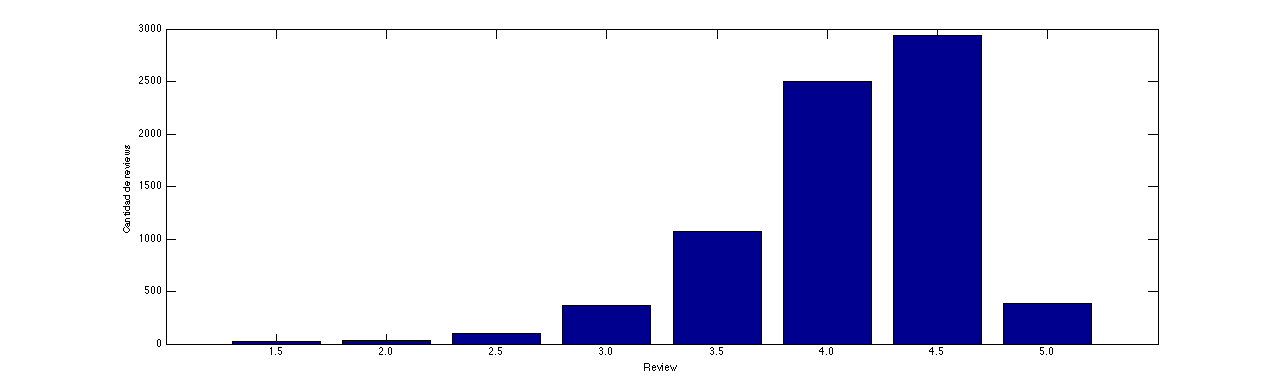
\includegraphics[width=8.0in]{imgs/grafDeBarras.png}
  \caption{Cantidad de reviews por puntaje}
\end{figure} 

\begin{figure}[H]
\begin{center}
  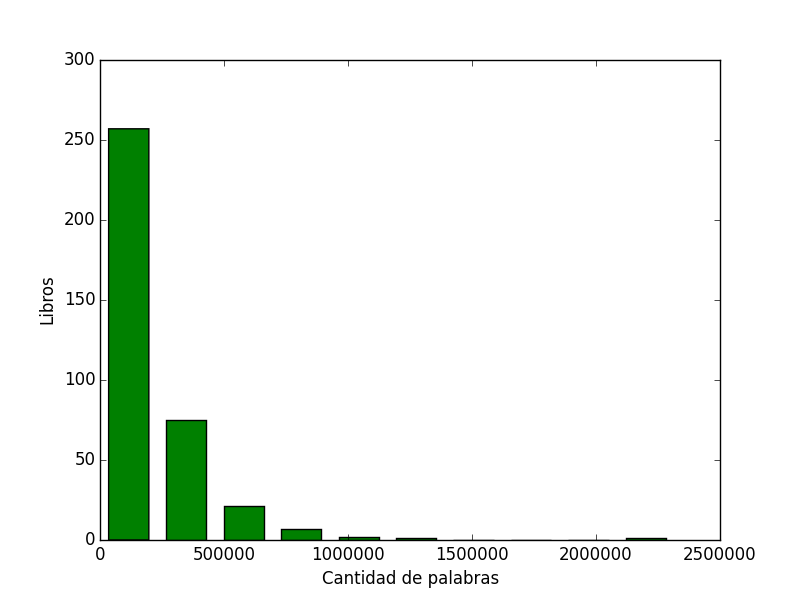
\includegraphics[width=6.0in]{../unigrams/scripts/histogram/histogramaDePalabras.png}
  \caption{Histograma de palabras}
  \end{center}
\end{figure}


\begin{figure}[H]
  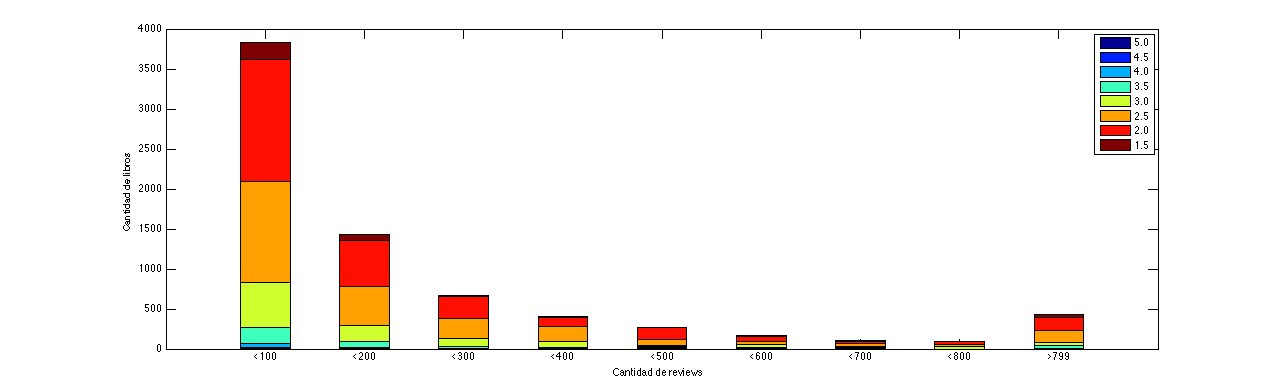
\includegraphics[width=8.0in]{imgs/cantLibrosVScantReviews.png}
  \caption{Cantidad de Libros vs cantidad de reviews}
\end{figure}

%Ademas hay que explicar cuantos libros agarramos de cada categoria principal y porque decidimos dejar los que tenian menos de 100 reviews fuera (basicamente, es por la convergencia del promedio de una muestra). \subsection{Resultados de las métricas} Podemos mostrar graficos de histogramas combinados, uno para los resultados de los libros ``Buenos'' y otros para los ``Malos'' de las 3 metricas: cantidad de palabras simple english, cantidad de vocabulario simple english y cantidad de repeticiones. Podemos decir que en un principio decidimos eliminar la cantidad de palabras como una metrica ya que da siempre entre 40\% y 50\% para todos los libros.\\

Luego, procedimos a descargar los libros, tarea que resultó altamente dificultosa para las obras poco populares o de bajo puntaje dada la falta de interés a digitalizarlos. La selección de los mismos se realizó como se explica a continuación.

\section{Experimentos y Resultados}

\subsection{Análisis de Resultados}

\begin{minipage}{\linewidth}
  \centering
  \begin{minipage}{0.25\linewidth}
      \begin{figure}[H]
          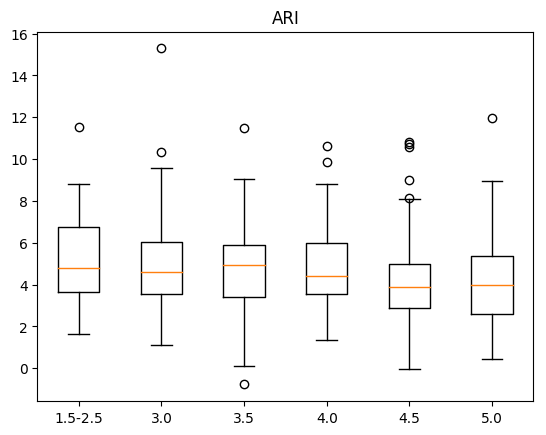
\includegraphics[width=2.3in]{../unigrams/scripts/boxplots/not-normalized-ARI.png}
          \caption{ARI}
      \end{figure}
  \end{minipage}
  \hspace{0.05\linewidth}
  \begin{minipage}{0.25\linewidth}
      \begin{figure}[H]
          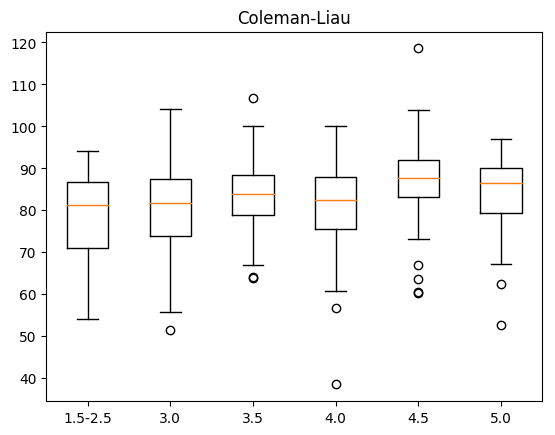
\includegraphics[width=2.3in]{../unigrams/scripts/boxplots/not-normalized-Coleman-Liau.png}
          \caption{Coleman-Liau}
      \end{figure}
  \end{minipage}
  \hspace{0.05\linewidth}
  \begin{minipage}{0.25\linewidth}
      \begin{figure}[H]
          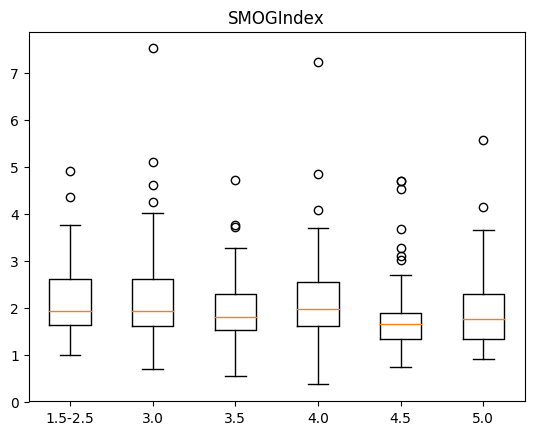
\includegraphics[width=2.3in]{../unigrams/scripts/boxplots/not-normalized-SMOGIndex.png}
          \caption{SMOGIndex}
      \end{figure}
  \end{minipage}
\end{minipage}

\begin{minipage}{\linewidth}
  \centering
  \begin{minipage}{0.25\linewidth}
      \begin{figure}[H]
          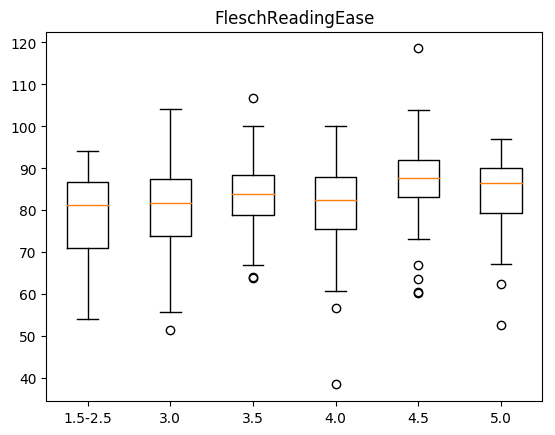
\includegraphics[width=2.3in]{../unigrams/scripts/boxplots/not-normalized-FleschReadingEase.png}
          \caption{FleschReadingEase}
      \end{figure}
  \end{minipage}
  \hspace{0.05\linewidth}
  \begin{minipage}{0.25\linewidth}
      \begin{figure}[H]
          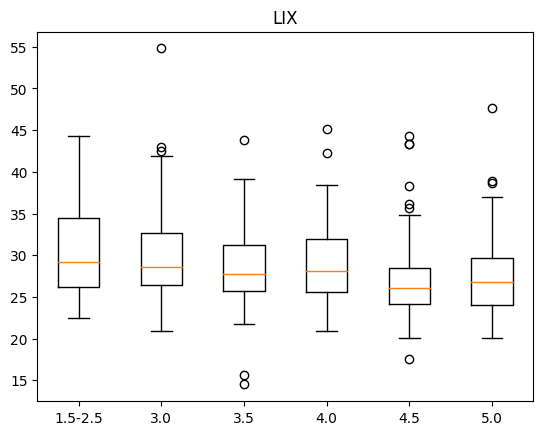
\includegraphics[width=2.3in]{../unigrams/scripts/boxplots/not-normalized-LIX.png}
          \caption{LIX}
      \end{figure}
  \end{minipage}
  \hspace{0.05\linewidth}
  \begin{minipage}{0.25\linewidth}
      \begin{figure}[H]
          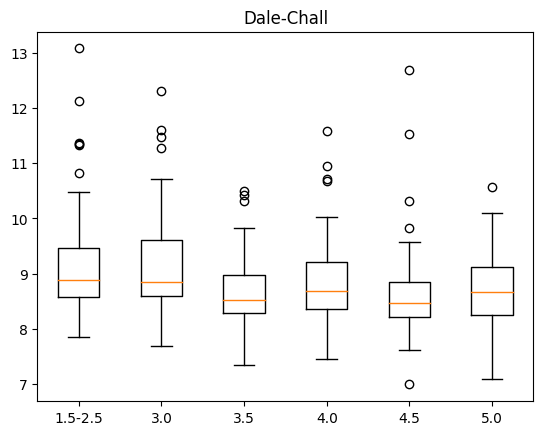
\includegraphics[width=2.3in]{../unigrams/scripts/boxplots/not-normalized-Dale-Chall.png}
          \caption{Dale-Chall}
      \end{figure}
  \end{minipage}
\end{minipage}

\subsection{Análisis de los Resultados del Test de Hipótesis}

Para plantear los Test de Hipótesis correspondientes, utilizamos la función $ks\_2samp$\footnote{https://docs.scipy.org/doc/scipy-0.15.1/reference/generated/scipy.stats.ks\_2samp.html} de la librería scipy que computa el estadístico Kolmogorov-Smirnov dadas dos muestras. Éste sirve para plantear el test de hipótesis nula que evalúa que dos muestras independientes se consiguen de la misma distribución continua.\\

Luego, dados dos arreglos \textbf{a} y \textbf{b} se obtienen \textbf{D} (o estadístico KS) y el p-valor correspondiente a \textbf{D}. El estadístico consiste en
$$D_{n}=\sup_{x}|F_{n}(x)-F(x)|$$
siendo $F(x)$ la función de distribución acumulada. Luego, si el estadístico KS es pequeño o el p-valor grande, no podemos rechazar la hipótesis de que las dos muestras son de la misma distribución.\footnote{https://ocw.mit.edu/courses/mathematics/18-443-statistics-for-applications-fall-2006/lecture-notes/lecture14.pdf}\\

La Hipótesis nula es rechazada con nivel $\alpha$ si $$D > c(\alpha) \cdot \sqrt{\frac{n_1+n_2}{n_1\cdot n_2}}$$ donde $n_1$ y $n_2$ son los tamaños de las muestras a comparar. El valor de $c(\alpha)$ se define como:
$$c(\alpha) = \sqrt{1/2\cdot log(\alpha/2)}$$

Los resultados obtenidos con un nivel de significancia de 0.001 para las métricas analizadas fueron los siguientes:\\

\begin{tabular}{ | l | l | l | l | }
\hline
Métrica & P-valor & D & Decisión sobre la Hipótesis nula\\
\hline
ARI & 1.9e-2 & 1.929e-2 & \textbf{NO rechazada} (1.9e-2 $<$ 0.001 y 2.5e-2 $<$ 1.929e-2)\\
\hline
LIX & 1.684e-3 & 2.378e-1 & \textbf{NO rechazada} (1.684e-3 $<$ 1e-3 y 2.5e-1 $<$ 2.378e-1)\\
\hline
Coleman-Liau & 5.97e-4 & 2.546e-1 & \textbf{Rechazada} (5.97e-4 $<$ 1e-3 y 2.5e-1 $<$ 2.546e-1)\\
\hline
FleschReadingEase & 9.126e-05 & 2.82e-1 & \textbf{Rechazada} (9.126e-05 $<$ 1e-3 y 2.5e-1 $<$ 2.82e-1)\\
\hline
Dale-Chall & 2.52e-05 & 3e-1 & \textbf{Rechazada} (2.52e-05 $<$ 1e-3 y 2.5e-1 $<$ 3e-1)\\
\hline
SMOGIndex & 8.01e-06 & 3.15e-1 & \textbf{Rechazada} (8.01e-06 $<$ 0.001 y 2.5e-1 $<$ 3.15e-1)\\
\hline
\end{tabular}


\section{Conclusiones y trabajo futuro} Por lo que vi vamos a tener que decir que obtuvimos resultados significativos pero los numeros estan demasiado cercanos como para utilizar la metrica como criterio. Explicar que otras metricas se nos ocurren para lo cual podria funcionar. Por ejemplo, a mi se me ocurre que una metrica mutli-variable con elementos de procesamiento de lenguaje natural podria dar mejores resultados, es decir metricas que describan mejor la forma en que el libro esta escrito.\\

%\begin{figure}[!t]
%\centering
%\includegraphics[width=2.5in]{myfigure}
% where an .eps filename suffix will be assumed under latex, 
% and a .pdf suffix will be assumed for pdflatex; or what has been declared
% via \DeclareGraphicsExtensions.
%\caption{Simulation Results.}
%\label{fig_sim}  
%\end{figure}

% An example of a double column floating figure using two subfigures.
% (The subfig.sty package must be loaded for this to work.)
% The subfigure \label commands are set within each subfloat command,
% and the \label for the overall figure must come after \caption.
% \hfil is used as a separator to get equal spacing.
% Watch out that the combined width of all the subfigures on a 
% line do not exceed the text width or a line break will occur.
%
%\begin{figure*}[!t]
%\centering
%\subfloat[Case I]{\includegraphics[width=2.5in]{box}%
%\label{fig_first_case}}
%\hfil
%\subfloat[Case II]{\includegraphics[width=2.5in]{box}%
%\label{fig_second_case}}
%\caption{Simulation results.}
%\label{fig_sim}
%\end{figure*}


% An example of a floating table. Note that, for IEEE style tables, the 
% \caption command should come BEFORE the table. Table text will default to
% \footnotesize as IEEE normally uses this smaller font for tables.
% The \label must come after \caption as always.
%
%\begin{table}[!t]
%% increase table row spacing, adjust to taste
%\renewcommand{\arraystretch}{1.3}
% if using array.sty, it might be a good idea to tweak the value of
% \extrarowheight as needed to properly center the text within the cells
%\caption{An Example of a Table}
%\label{table_example}
%\centering
%% Some packages, such as MDW tools, offer better commands for making tables
%% than the plain LaTeX2e tabular which is used here.
%\begin{tabular}{|c||c|}
%\hline
%One & Two\\
%\hline
%Three & Four\\
%\hline
%\end{tabular}
%\end{table}


%\ifCLASSOPTIONcaptionsoff
%  \newpage
%\fi


\begin{thebibliography}{1}

\bibitem{hu} Nan Hu, Paul A Pavlou, and Jennifer Zhang, ``Can online reviews reveal a product’s true quality?: empirical findings and analytical modeling of online wordof-mouth communication,''\hskip 1em plus
  0.5em minus 0.4em\relax in \emph{Proceedings of the 7th ACM conference on Electronic commerce}. ACM, 2006, pp. 324–330.
  
\bibitem{talwar} Arjun Talwar, Radu Jurca, and Boi Faltings, ``Understanding user behavior in online feedback reporting,''\hskip 1em plus
  0.5em minus 0.4em\relax in \emph{Proceedings of the 8th ACM conference on Electronic commerce}. ACM, 2007, pp. 134–142.

\bibitem{muchnik} Lev Muchnik, Sinan Aral, and Sean J Taylor,``Social influence bias: A randomized experiment,''\hskip 1em plus
  0.5em minus 0.4em\relax \emph{Science, vol. 341(6146)}, pp. 647–651, August 2013.

\bibitem{zhang}
Zhang, Yaonan, et al. ``Online ratings: Convergence towards a positive perspective?.'' \hskip 1em plus
  0.5em minus 0.4em\relax \emph{Acoustics, Speech and Signal Processing (ICASSP)}, 2014 IEEE International Conference on. IEEE, 2014.

\bibitem{chevalier}
Judith A Chevalier and Dina Mayzlin, ``The effect of word of mouth on sales: Online book reviews,'' \hskip 1em plus
  0.5em minus 0.4em\relax \emph{Journal of marketing research}, vol. 43, pp. 354–54, August 2006.

\bibitem{fowler}
G. A. Fowler and J.D. Avila, ``On the internet, everyone’s a critic but they’re not very critical,'' \hskip 1em plus
  0.5em minus 0.4em\relax \emph{Wall Street Journal}, 2009.

\bibitem{leskovec}
J. Leskovec, L. Adamic and B. Adamic. ``The Dynamics of Viral Marketing''.\hskip 1em plus
  0.5em minus 0.4em\relax \emph{ACM Transactions on the Web (ACM TWEB)}, 1(1), 2007.

\bibitem{graesser}
Graesser,~A.~C.,~McNamara,~D.~S.,~Louwerse,~M.~M., \& Cai,~Z. (2004). ``Coh-Metrix: Analysis of text on cohesion and language.''\footnote{http://cor.to/graesser} \hskip 1em plus
  0.5em minus 0.4em\relax \emph{Behavior Research Methods,Instruments, \& Computers}, 36(2), 193-202.

\bibitem{crossley}
Crossley,~S.~A.,~Allen,~D.~B., \& McNamara,~D.~S. (2011). ``Text Readability and Intuitive Simplification: A Comparison of Readability Formulas.''\hskip 1em plus
  0.5em minus 0.4em\relax \emph{Reading in a foreign language}, 23(1), 84-101.

\bibitem{diuk}
Diuk,~C.~G.,~Slezak,~D.~F.,~Raskovsky,~I.,~Sigman,~M., \& Cecchi,~G.~A. (2012). ``A quantitative philology of introspection.''\hskip 1em plus
  0.5em minus 0.4em\relax \emph{Frontiers in integrative neuroscience}, 6.
  
\bibitem{orlow} 
Paasche-Orlow MK, Taylor HA, Brancati FL (2003)`` Readability standards for informed-consent forms as compared with actual readability''.\hskip 1em plus
  0.5em minus 0.4em\relax \emph{New England Journal of Medicine} 348: 721–726.
  
\bibitem{klare} 
Klare GR (1974) ``Assessing readability''.\hskip 1em plus
  0.5em minus 0.4em\relax \emph{Reading Research Quarterly} 10: 62–102.
  
\bibitem{kanungo} 
Kanungo T, Orr D (2009) ``Predicting the readability of short web summaries''.\hskip 1em plus
  0.5em minus 0.4em\relax \emph{Proceedings of the Second ACM International Conference on Web Search and Data Mining} (WSDM ’09). New York: ACM Press. 202–211.
  
\bibitem{karmakar} 
Karmakar S, Zhu Y (2010) ``Visualizing multiple text readability indexes''.\hskip 1em plus
  0.5em minus 0.4em\relax \emph{2010 International Conference on Education and Management Technology} (ICEMT). Washington, DC: IEEE. 133–137.

\bibitem{izgi} 
Izgi, Umit, and Burcu Sezginsoy Seker. ``Comparing different readability formulas on the examples of science-technology and social science textbooks.''\hskip 1em plus
  0.5em minus 0.4em\relax \emph{Procedia-Social and Behavioral Sciences} 46 (2012): 178-182.
  
\bibitem{smog}
Mc Laughlin, G. Harry. ``SMOG grading-a new readability formula.''\hskip 1em plus
  0.5em minus 0.4em\relax \emph{Journal of reading 12.8} (1969): 639-646.

\bibitem{ari-flesch}
Kincaid, J. Peter, et al. ``Derivation of new readability formulas (automated readability index, fog count and flesch reading ease formula) for navy enlisted personnel.''\hskip 1em plus
  0.5em minus 0.4em\relax No. RBR-8-75. \emph{Naval Technical Training Command Millington TN Research Branch}, 1975.

\bibitem{lix-rix}
Anderson, Jonathan. ``Lix and rix: Variations on a little-known readability index.''\hskip 1em plus
  0.5em minus 0.4em\relax \emph{Journal of Reading} 26.6 (1983): 490-496.

\bibitem{coleman-liau}
Coleman, Meri, and Ta Lin Liau. ``A computer readability formula designed for machine scoring.''\hskip 1em plus
  0.5em minus 0.4em\relax \emph{Journal of Applied Psychology} 60.2 (1975): 283.

\bibitem{dale-chall}
Dale, Edgar, and Jeanne S. Chall. ``A formula for predicting readability: Instructions.''\hskip 1em plus
  0.5em minus 0.4em\relax \emph{Educational research bulletin} (1948): 37-54.

\bibitem{dale-chall-ex}
Chall, Jeanne Sternlicht, and Edgar Dale. ``Readability revisited: The new Dale-Chall readability formula.''\hskip 1em plus
  0.5em minus 0.4em\relax \emph{Brookline Books}, 1995.
  
\bibitem{liang} 
Liang, Franklin Mark. Word Hy-phen-a-tion by Com-put-er. \hskip 1em plus
  0.5em minus 0.4em\relax \emph{Department of Computer Science, Stanford University}, 1983.
  
\bibitem{hedman}
Hedman, Amy S. ``Using the SMOG formula to revise a health-related document.'' \hskip 1em plus
  0.5em minus 0.4em\relax \emph{American Journal of Health Education} 39.1 (2008): 61-64.

\end{thebibliography}

\end{document}


